En este pasaje se mostrarán los diagramas de estados del sistema.
Se puede notar que el sistema cuenta con 4 estados distintivos, siendo estos
\begin{itemize}
\item Initial
\item Idle
\item Charging
\item Communicating
\end{itemize}
Cabe la pena mencionar que en cualquiera de los estados salvando por el incial, el sistema estará realizando mediciones del ambiente, al igual de tener la posibilidad de comunicarse por Bluetooth con la electrónica de la mochila. \footnote{A menos que el nivel de carga de la UBM no sea suficiente.}

\begin{figure}[H]
	\centering
	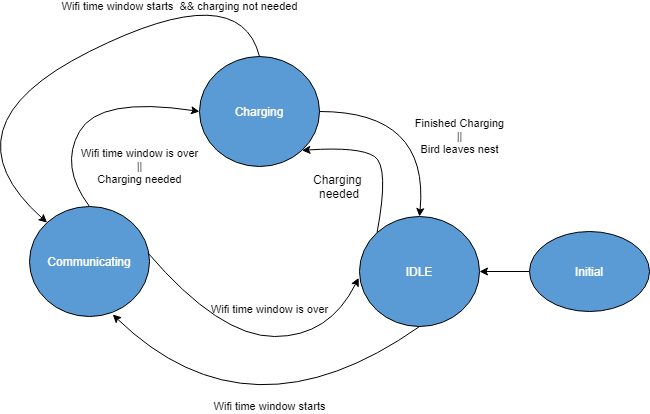
\includegraphics[width=0.9\linewidth]{ImagenesIngenieria de Detalle/Diagrama_de_Estados}
	\label{fig:Diagrama_de_Estados}
	\caption{Diagrama de estados.}
\end{figure}

En el estado ``Initial'' es aquel donde se inicializan todos los drivers, estructuras de datos y configuraciones iniciales, no se volverá a este estado una vez que este haya sido abandonado. 

\begin{figure}[H]
	\centering
	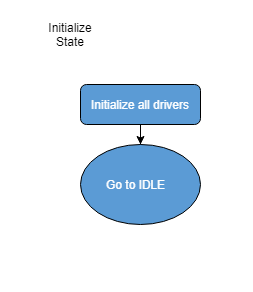
\includegraphics[width=0.4\linewidth]{ImagenesIngenieria de Detalle/diagrama_flujo_initial}
	\label{fig:Diagrama_de_flujo_init}
	\caption{Diagrama de flujo: Estado ``Initial''.}
\end{figure}
Luego se encuentra el estado ``IDLE'' en este estado se sensaran las variables fisicas con el periodo de muestreo acorde a cada especificado en \note{PONER LUGAR DONDE ESTE ESPECIFICADO ESTO}
luego se fijará si es momento de prender el hotspot wifi, si es asi irá al estado ``Communicating''. Si no es as\'i se ver\'a si hay que cargar la bater\'ia, en caso positivo ir\'a a estado ``Charging'', caso contrario se corrobora si hay transmisi\'on Bluetooth, actua acorde  y comienza el ciclo nuevamente.
\begin{figure}[H]
	\centering
	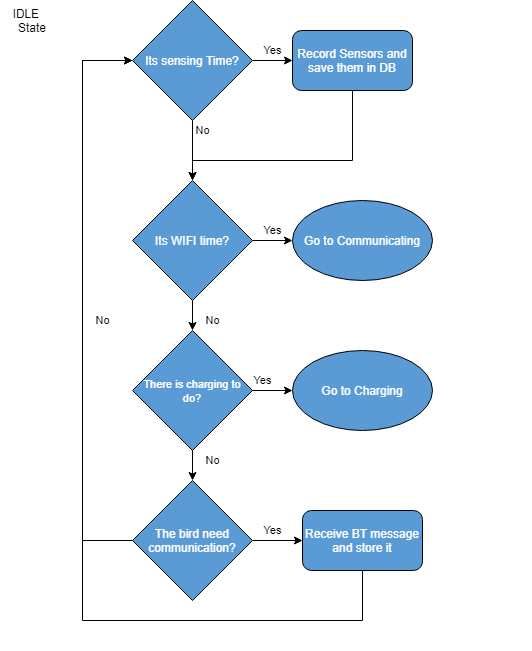
\includegraphics[width=0.9\linewidth]{ImagenesIngenieria de Detalle/diagrama_flujo_idle}
	\label{fig:Diagrama_de_flujo_idle}
	\caption{Diagrama de flujo: Estado ``IDLE''.}
\end{figure}
En el estado ``Charging'' su funci\'on principal ser\'a la de cargar la UBM. Lo primero a hacer en este estado es habilitar el cargador, luego si hay un mensaje Bluetooth, se comienza la comunicaci\'on y se recibe hasta que esta haya terminado. A continuaci\'on se encarga del sensado, luego se verifica si la carga termin\'o, si es as\'i se desactiva el cargador, y dependiendo si es momento de habilitar el hotspot o no se ir\'a al estado ``Communicating'' \'o ``IDLE''
\begin{figure}[H]
	\centering
	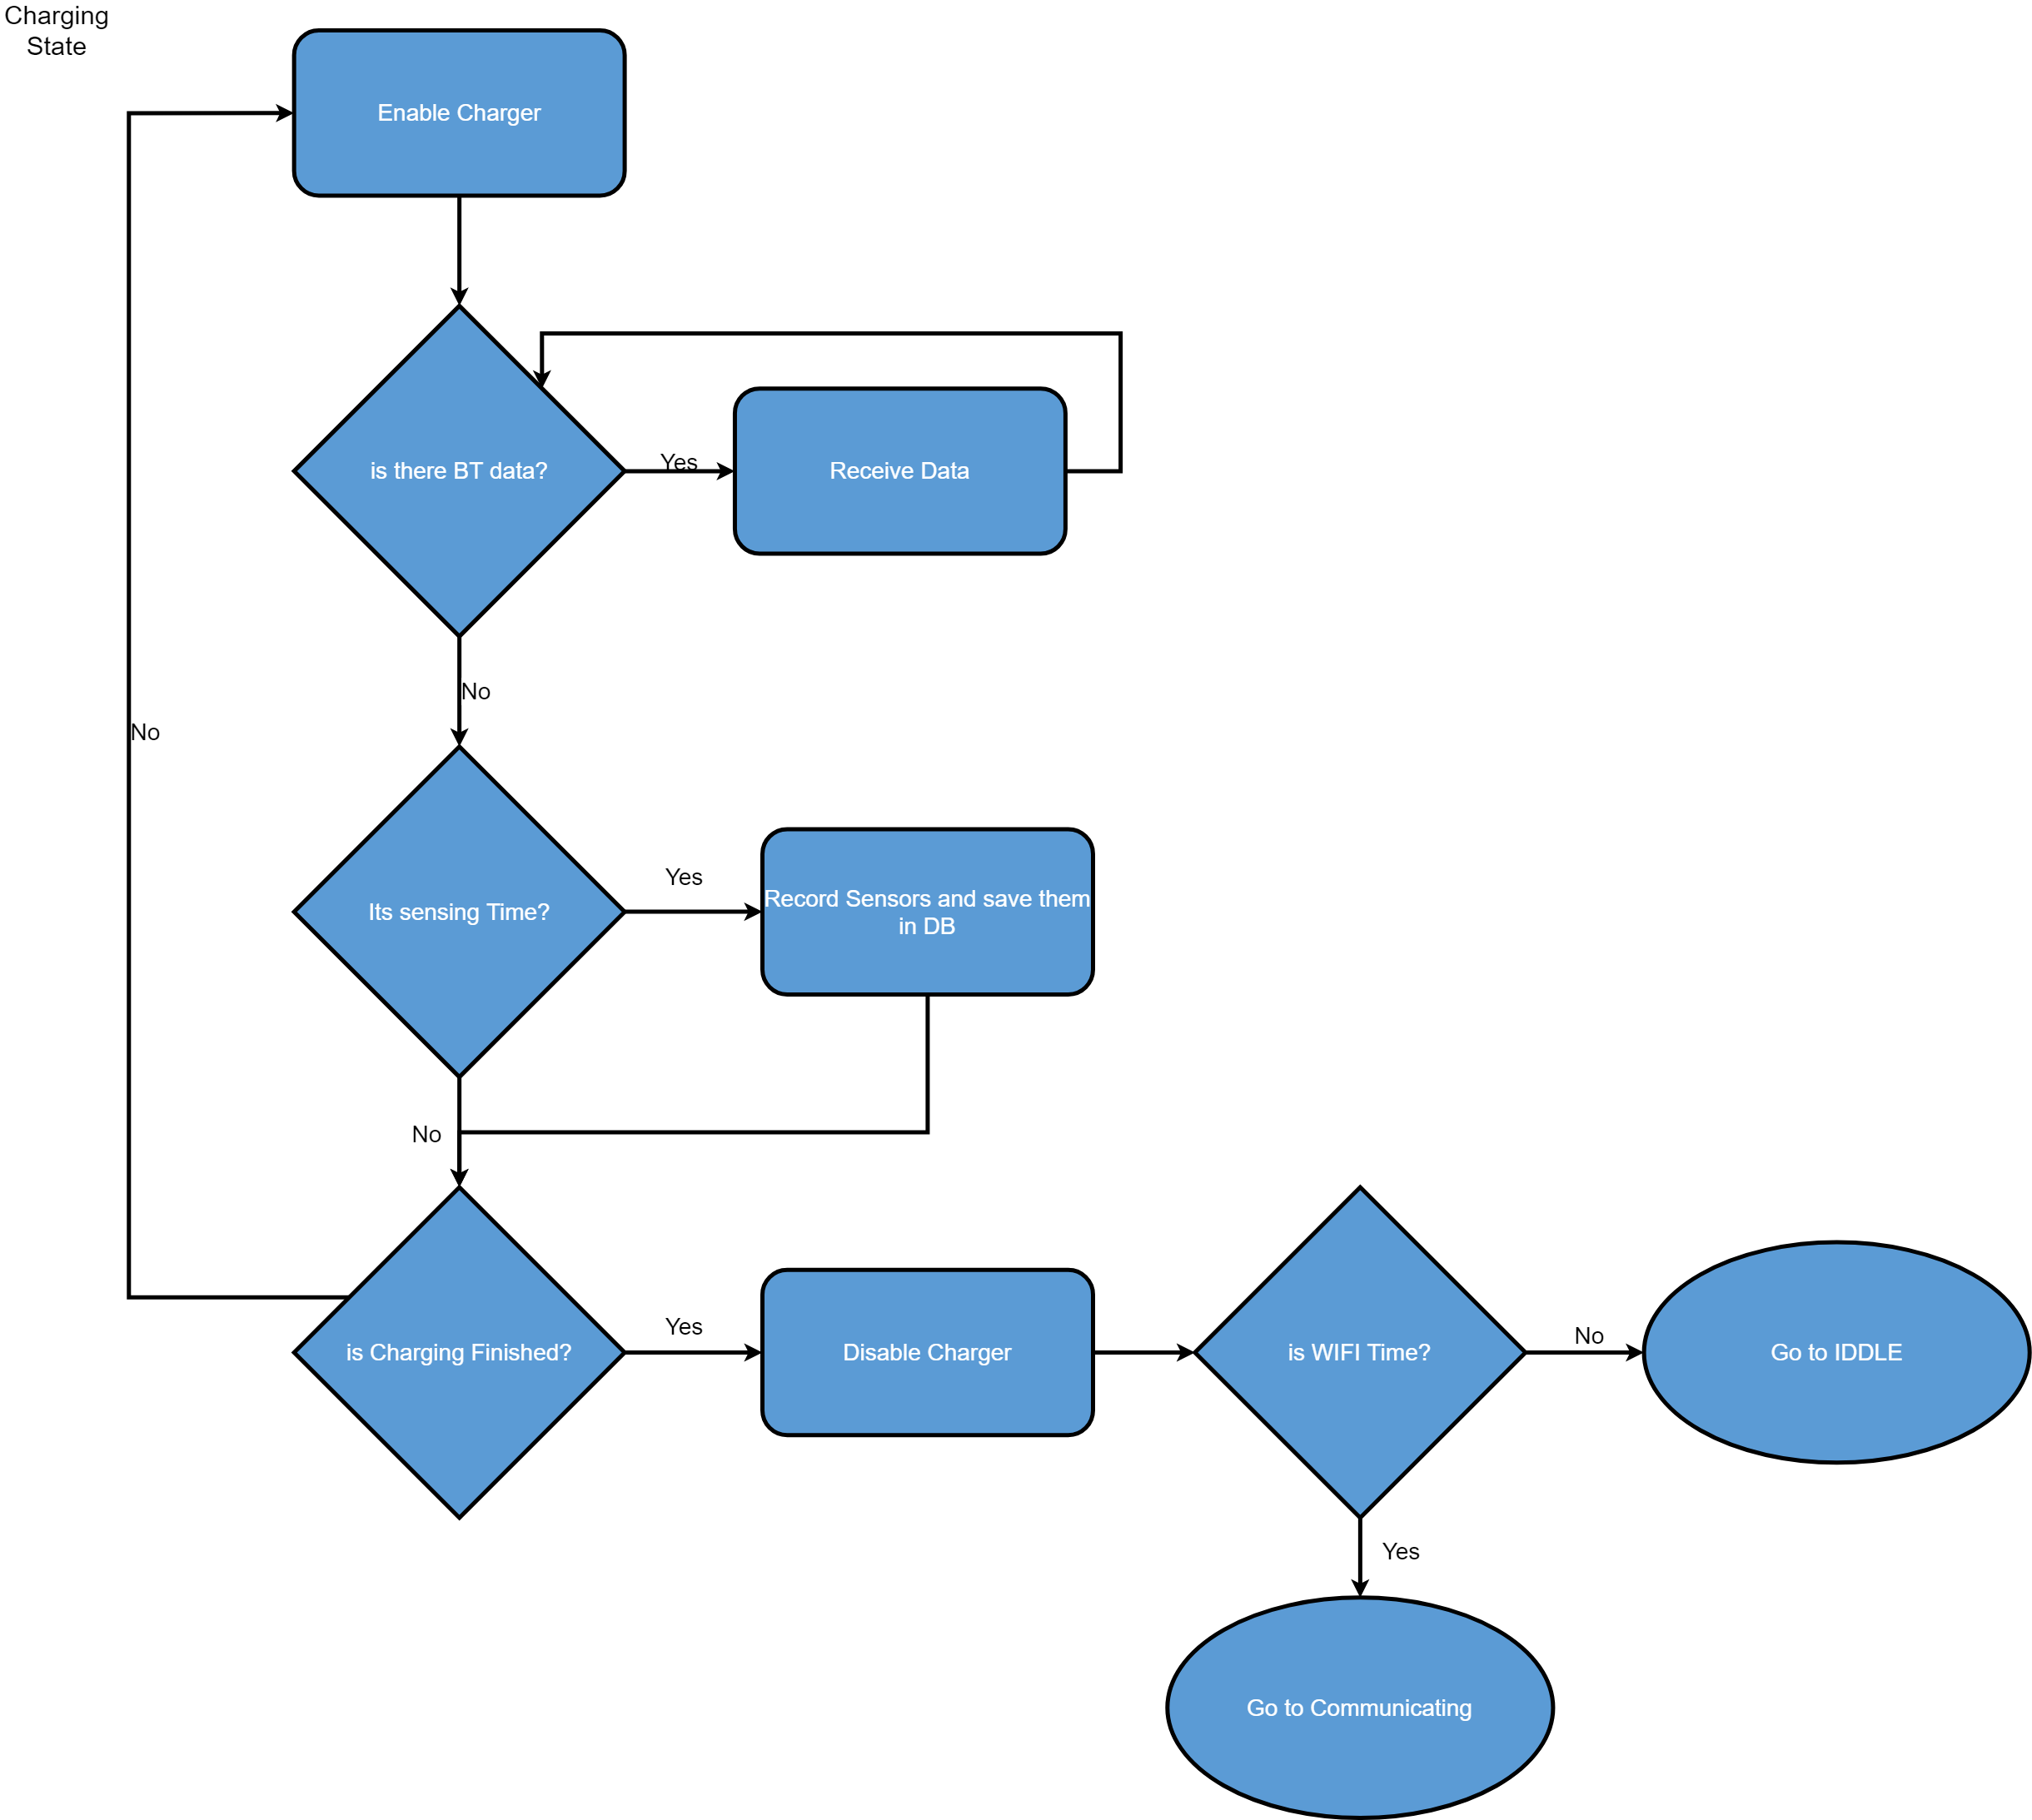
\includegraphics[width=0.9\linewidth]{ImagenesIngenieria de Detalle/diagrama_flujo_charging}
	\label{fig:Diagrama_de_flujo_charging}
	\caption{Diagrama de flujo: Estado ``Charging''.}
\end{figure}
Finalmente en el estado ``Communicating'' es aquel en el que se habilita el hotspot y se levanta el servidor de Node-red, aqui se comunica el nido con una computadora en al base del nido, esto se mantendr\'a hasta que haya pasado el tiempo especificado en \note{No se deberiamos decirlo en algun lado, probablemente hardware}. Ademas se continuan sensando las variables f\'isicas
\begin{figure}[H]
	\centering
	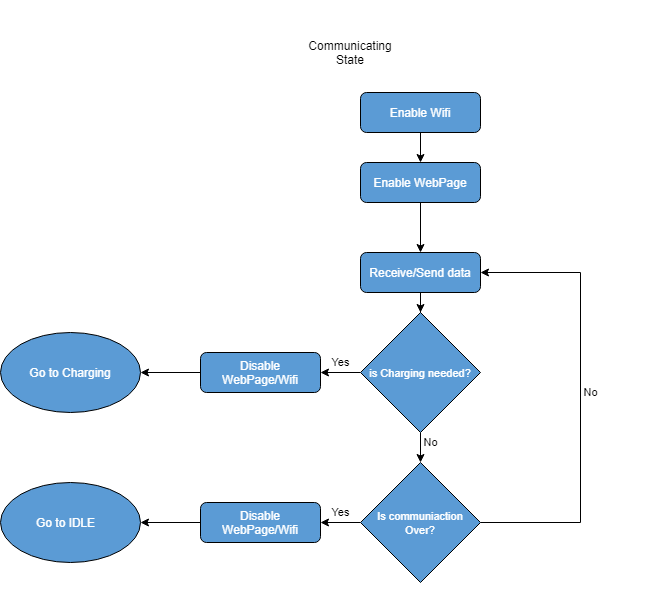
\includegraphics[width=0.9\linewidth]{ImagenesIngenieria de Detalle/diagrama_flujo_communicating}
	\label{fig:diagrama_flujo_communicating}
	\caption{Diagrama de flujo: Estado ``Communicating''.}
\end{figure}